\documentclass[12pt]{article}
\usepackage[margin=0.5in]{geometry}
\usepackage{float}
\usepackage{amsmath} %used for align environment
\usepackage{titlesec} %used to format titles
\usepackage{graphicx} %for handling figures
\usepackage[none]{hyphenat} %disallows hyphenated words
\usepackage[labelformat=empty]{caption} %removes figure numbering


\begin{document}

\pagestyle{empty}

\titleformat{\section}{\normalfont\small\bfseries}{\thesection}{1em}{} 
\titleformat{\subsection}{\normalfont\small\bfseries}{\thesection}{1em}{} 

\section*{Power Spectra \\Lecture: Adrian Liu \\Notes: Carina Cheng \\7/2/14}

\subsection*{More on Power Spectra}

Last lecture, we derived the expression for a power spectrum, which is represented by the average of the fourier temperature squared. In other words, a power spectrum is a variance on various k-scales.
\begin{align} \label{eq: pspec}
\langle \tilde{T}(\boldsymbol{k}) \tilde{T}^{\ast}(\boldsymbol{k'}) \rangle &= (2\pi)^{3}\delta^{D}(\boldsymbol{k}-\boldsymbol{k'})P(\boldsymbol{k})
\end{align}

\noindent Also recall the fourier transform definitions used in the derivation.
\begin{align} \label{eq: ft}
\tilde{T}(\boldsymbol{k}) &= \int d^{3}\boldsymbol{r}e^{-i\boldsymbol{k}\cdot \boldsymbol{r}} \ T(\boldsymbol{r}) \\
\label{eq: ift}
T(\boldsymbol{r}) &= \int {\frac{d^{3}\boldsymbol{k}}{(2\pi)^{3}}}e^{-i\boldsymbol{k}\cdot \boldsymbol{r}} \ \tilde{T}(\boldsymbol{k})
\end{align}

\noindent Let's examine the units of the various components in these expressions. The delta function in equation \ref{eq: pspec} has units of $\Big[{\frac{1}{x}}\Big]$ because $1 = \int \delta(x) dx$. Therefore, $\Big[\delta(\boldsymbol{k})\Big] \sim \Big[x^{3}\Big]$, since $k$ has units of inverse length and we are working with three dimensions. So effectively, $\delta(\boldsymbol{k})$ is a volume, and therefore $P(\boldsymbol{k}) \propto {\frac{\langle |\tilde{T}(\boldsymbol{k})|^{2}\rangle}{volume}}$. The fourier transform of the sky, $\tilde{T}(\boldsymbol{k})$ typically has units of $\Big[mK \cdot Mpc^{3}\Big]$ because of equation \ref{eq: ft} and then it follows that the power spectrum $P(\boldsymbol{k})$ has units of $\Big[mK^{2} \cdot Mpc^{3}\Big]$. \\

\noindent The following is a recipe for obtaining a power spectrum of the sky: \\ \\
i) Start with $T(\boldsymbol{r})$, a temperature distribution of the sky \\
ii) Fourier transform to get $\tilde{T}(\boldsymbol{k})$ \\
iii) Square $\tilde{T}(\boldsymbol{k})$ to get $|\tilde{T}(\boldsymbol{k})|^{2}$ \\
iv) Bin in constant contours of $k$ \\

\noindent One thing to note is that we can apply the cosmological principle that the Universe is isotropic on large scales (that is, looks the same in every direction). So even if we measure different sky temperatures in different directions, the statistics will be the same because of isotropy. Recall that the power spectrum is just the variance of a particular Fourier mode. In an isotropic Universe, the variance is a function of $k$ instead of $\boldsymbol{k}$, making $P(\boldsymbol{k})$ easier to measure (can bin over different $k$ to increase S/N). However, $\tilde{T}(\boldsymbol{k})$ is random, as well as $\hat{p}(\boldsymbol{k})$ (an estimate of $P(\boldsymbol{k})$; errors in $P(\boldsymbol{k})$ measurements), so the trick of isotropy is invalid for those quantities. \\

\noindent For high k-modes, there are more samples along the constant k contours. Therefore, high k-modes are more reliable estimates of the power spectrum, but only if noise is not an issue. As you move to lower and lower k-modes, there are fewer samples and you eventually approach a fundamental limit of having too few modes of the Universe to measure. This phenomenon is called `cosmic variance.' It is a good thing to be cosmic variance limited because it means that your instrument is performing at its best and isn't noise-dominated, but on the other hand it means that you can't make improvements to your power spectrum anymore. \\

\noindent When noise is the limiting factor, such as for PAPER, it is ideal to have $N$ baselines of the same lengths and orientation, all measuring the same fourier mode with the same sky temperature. This redundant sampling is a way to build up signal and minimize errors. Following traditional statistics (if combining $N$ independent measurements to measure a single number, the error in that number goes down like $1/\sqrt{N}$), the error for the fourier transform of temperature is the following:
\begin{align}
\Delta \tilde{T}(k) &\sim {\frac{1}{\sqrt{N}}} 
\end{align}

\noindent And since $P \propto \tilde{T}(k)^{2}$ (from equation \ref{eq: pspec}):
\begin{align}
\Delta P &\sim {\frac{1}{N}}
\end{align}

\noindent However, in the case of $N$ baselines of the same lengths but at different orientations, the baselines measure different fourier modes (different temperatures). But due to statistical isotropy, the baselines measure the same power spectrum. So combining $N$ power measurements yields the following error. Note that this error is larger than in the previous case. 
\begin{align}
\Delta P &\sim {\frac{1}{\sqrt{N}}}
\end{align}

\noindent The two different errors on power essentially depend on when you're allowed to combine measurements. If you're combining after making temperature measurements, the errors on temperature decrease as $1/\sqrt{N}$, but if you're combining after making power measurements, the errors on power decrease as $1/\sqrt{N}$. \\

\noindent Once the instrument hits $S/N \sim 1$ per fourier mode (per every value of k), cosmic variance comes into play. Hence, the interferometry-building strategy changes around this limit. If noise-dominated with low $S/N$, then redundant sampling is useful because you can beat down your noise better. \\ 

\noindent Sometimes in the literature it is common to see a different form of the power spectrum, with units of $\Big[mK^{2}\Big]$, and defined as:
\begin{align}
\Delta^{2}(\boldsymbol{k}) &= {\frac{k^{3}}{2\pi^{2}}}P(\boldsymbol{k})
\end{align}

\noindent Let's apply some of these concepts to reionization. When there's lots of fine initial structure in the Universe, high k-modes dominate the power (see Figure 1, dotted curve). However, as ionization occurs, larger ionized bubbles begin to dominate the fine structure and therefore there becomes less high k-mode power and more low k-mode power (see Figure 1, solid curve). There is also an evolution of the power dropping as a whole over time since there is fundamentally less hydrogen to trace as it becomes ionized. Foreground sources, however, are smooth in frequency and dominate low k-modes. So for example, PAPER data produces a power spectrum that increases at low k's due to these foregrounds (see Figure 2). \\

\begin{figure}[H]
\centering
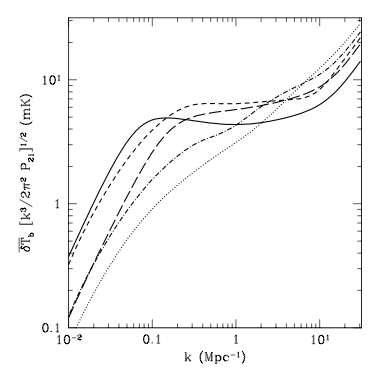
\includegraphics[totalheight=0.4\textheight]{furlanettoetal.png}
\caption{Fig. 1. RMS variation in the 21 cm brightness temperature as a function of wavenumber at several different stages of reionization (z=10). The curves have different ionization fractions which increase from the dotted curve, dash-dotted curve, short-dashed curve, long-dashed curve, to the solid curve. Figure from Furlanetto et al. 2006.}
\end{figure}

\begin{figure}[H]
\centering
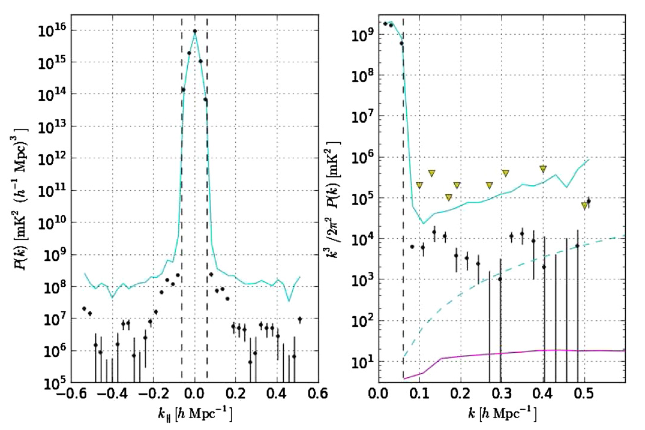
\includegraphics[totalheight=0.4\textheight]{parsonsetal.png}
\caption{Fig. 2. Power spectra at z=7.7 with 32 PAPER antennas. Figure from Parsons et al. 2014.}
\end{figure}

\subsection*{Power Spectra with Interferometers}

Now let's apply the power spectra basics to radio interferometry. Radio telescopes measure visibilities as a function of baseline coordinates and frequency:
\begin{align}
V\Big(\boldsymbol{u}={\frac{\boldsymbol{b}}{\lambda}},\nu \Big) &= \int dl \ dm \ T(\boldsymbol{\theta},\nu)A(\boldsymbol{\theta},\nu)e^{-i2\pi(ul+vm)}\Big({\frac{2k_{B}}{\lambda^{2}}}\Big)
\end{align}

\noindent $T(\boldsymbol{\theta},\nu)$ is the sky temperature measured as a function of angle and frequency, and $A(\boldsymbol{\theta},\nu)$ is the beam response. The Rayleigh-Jeans factor tacked onto the end is used to convert from visibility units of Jansky's $\Big[{\frac{W}{m^{2}Hz}} = {\frac{kg}{s^{2}}}\Big]$ to temperature units. Notice that the interferometer already does two spatial fourier transforms of the sky temperature $T$ already. Recall that the phase term is $e^{-i2\pi {\frac{\boldsymbol{b} \cdot \hat{s}}{\lambda}}}$, where $u$ and $v$ represent the east/west and north/south components of the baseline vector $\boldsymbol{b}$, and $l$ and $m$ represent the east/west and north/south components of the source direction unit vector $\hat{s}$. We can therefore just take the 3rd fourier transform of the frequency axis on our way to forming a power spectrum. \\

\noindent But first, let's do some unit conversions from angles on the sky to real physical distances. If we assume a flat sky and look at a small patch, the angles subtended $\theta_{x}$ and $\theta_{y}$ are related to $l$ and $m$ by:
\begin{align}
l \sim sin\theta_{x} &\sim \theta_{x} \\
m \sim sin\theta_{y} &\sim \theta_{y}
\end{align}

\noindent If $x$ and $y$ describe the size of the sky patch (in $Mpc$, for example), and $X$ is the cosmological distance to the patch, then:
\begin{align}
x &= X\theta_{x} \\
y &= X\theta_{y} \\
r_{los} &= Y\nu
\end{align}

\noindent The third expression is written similarly to the others but relates the line-of-sight size to frequency. Now we can go ahead and re-write the visibility equation using these physical coordinates.
\begin{align}
V\Big(\boldsymbol{u},\nu \Big) &= \int dx \ dy \ {\frac{1}{X^{2}}} \ T(\boldsymbol{r})A(\boldsymbol{r})e^{{\frac{-i2\pi(ux+vy)}{X}}}\Big({\frac{2k_{B}}{\lambda^{2}}}\Big)
\end{align}

\noindent And now let's do that third fourier transform along the frequency axis.
\begin{align}
\tilde{V}(\boldsymbol{u},\eta) &= \int d\nu \ e^{-i2\pi\eta\nu}V(\boldsymbol{u},\nu) \\
\tilde{V}(\boldsymbol{u},\eta) &= {\frac{1}{X^{2}Y}}\Big({\frac{2k_{B}}{\lambda^{2}}}\Big) \int d^{3}\boldsymbol{r} \ T(\boldsymbol{r}) A(\boldsymbol{r})e^{-i\boldsymbol{k} \cdot \boldsymbol{r}} \\
\boldsymbol{k} &= (k_{x},k_{y},k_{z}) = \Big({\frac{2\pi u}{X}},{\frac{2\pi v}{X}},{\frac{2\pi \eta}{Y}}\Big)
\end{align}

\noindent So essentially, we used coordinate relationships to go from $(l, m, \nu)$ to $(x, y, r_{los})$ and fourier transformed $(l, m, \nu)$ to $(u, v, \eta)$. Every baseline of an interferometer measures a point in the u-v plane (one fourier mode). \\

\noindent Now we convolve $\tilde{T}(\boldsymbol{k})$ with $\tilde{A}(\boldsymbol{k})$ by first plugging in equation \ref{eq: ift} for $T(\boldsymbol{r})$ (using the dummy variable $\boldsymbol{k_{a}}$) and similarly for $A(\boldsymbol{r})$ (using the dummy variable $\boldsymbol{k_{b}}$), and applying the following trick:
\begin{align} \label{eq: deltatrick}
\int d^{3}\boldsymbol{r} e^{i(\boldsymbol{k_{a}}+\boldsymbol{k_{b}} - \boldsymbol{k}) \cdot \boldsymbol{r}} &= \delta (\boldsymbol{k_{a}}+\boldsymbol{k_{b}} - \boldsymbol{k}) (2\pi)^{3}
\end{align}

\noindent The result of this convolution is the following:
\begin{align}
\tilde{V}(\boldsymbol{u},\eta) &= {\frac{1}{X^{2}Y}}\Big({\frac{2k_{B}}{\lambda^{2}}}\Big) \int {\frac{d^{3}\boldsymbol{k_{a}}}{(2\pi)^{3}}} \tilde{A}(\boldsymbol{k}-\boldsymbol{k_{a}}) \tilde{T}(\boldsymbol{k_{a}})
\end{align}

\noindent Let's apply this convolution:
\begin{align}
\langle \tilde{V}(\boldsymbol{u},\eta) \tilde{V}^{\ast}(\boldsymbol{u'},\eta') \rangle &= \bigg[{\frac{1}{X^{2}Y}}\Big({\frac{2k_{B}}{\lambda^{2}}}\Big)\bigg]^{2} \int {\frac{d^{3}\boldsymbol{k_{a}}}{(2\pi)^{3}}} {\frac{d^{3}\boldsymbol{k_{b}}}{(2\pi)^{3}}} \tilde{A}(\boldsymbol{k}-\boldsymbol{k_{a}}) \tilde{A}^{\ast}(\boldsymbol{k'}-\boldsymbol{k_{b}}) \langle \tilde{T}(\boldsymbol{k_{a}})\tilde{T}^{\ast}(\boldsymbol{k_{b}})\rangle
\end{align}

\noindent And note from equation \ref{eq: pspec} that:
\begin{align}
\langle \tilde{T}(\boldsymbol{k_{a}})\tilde{T}^{\ast}(\boldsymbol{k_{b}})\rangle &= (2\pi)^{3} P(\boldsymbol{k_{a}}) \delta^{D}(\boldsymbol{k_{a}}-\boldsymbol{k_{b}})
\end{align}

\noindent Integrating over $\boldsymbol{k_{b}}$, the expression is only non-zero for $\boldsymbol{k_{a}} = \boldsymbol{k_{b}}$: 
\begin{align}
\langle \tilde{V}(\boldsymbol{u},\eta) \tilde{V}^{\ast}(\boldsymbol{u'},\eta') \rangle &= \bigg[{\frac{1}{X^{2}Y}}\Big({\frac{2k_{B}}{\lambda^{2}}}\Big)\bigg]^{2} \int {\frac{d^{3}\boldsymbol{k_{a}}}{(2\pi)^{3}}}  \tilde{A}(\boldsymbol{k}-\boldsymbol{k_{a}}) \tilde{A}^{\ast}(\boldsymbol{k'}-\boldsymbol{k_{a}}) P(\boldsymbol{k_{a}})
\end{align}

\noindent Now if we set $\boldsymbol{u} = \boldsymbol{u'}$ (if using the same baseline lengths) and $\eta = \eta'$, then $k = k'$ and the expression can be squared.
\begin{align}
\langle |\tilde{V}(\boldsymbol{u},\eta) |^{2} \rangle &= \bigg[{\frac{1}{X^{2}Y}}\Big({\frac{2k_{B}}{\lambda^{2}}}\Big)\bigg]^{2} \int {\frac{d^{3}\boldsymbol{k_{a}}}{(2\pi)^{3}}} |\tilde{A}(\boldsymbol{k}-\boldsymbol{k_{a}})|^{2}P(\boldsymbol{k_{a}})
\end{align}

\noindent For example, when making PAPER spectra with a wide beam, the power is broad and can be taken outside of the integral. This approximation is called the Feldman-Kaiser-Peacock (FKP) approximation. Note that it breaks down at low k-modes because of foregrounds though, when $P(k)$ rapidly increases.
\begin{align}
\langle |\tilde{V}(\boldsymbol{u},\eta) |^{2} \rangle &\sim P(\boldsymbol{k})  \bigg[{\frac{1}{X^{2}Y}}\Big({\frac{2k_{B}}{\lambda^{2}}}\Big)\bigg]^{2} \int {\frac{d^{3}\boldsymbol{k_{a}}}{(2\pi)^{3}}} |\tilde{A}(\boldsymbol{k}-\boldsymbol{k_{a}})|^{2}
\end{align}

\noindent Defining $q = k - k_{a}$:
\begin{align}
\langle |\tilde{V}(\boldsymbol{u},\eta) |^{2} \rangle &\sim P(\boldsymbol{k})  \bigg[{\frac{1}{X^{2}Y}}\Big({\frac{2k_{B}}{\lambda^{2}}}\Big)\bigg]^{2} \int {\frac{d^{3}q}{(2\pi)^{3}}} |\tilde{A}(q)|^{2}
\end{align}

\noindent Parseval's Theorem states that inner products do not depend on basis, so a change of basis such as a fourier transform should not affect an inner product. Let's apply this when going back to real space (using equation \ref{eq: ift} and a similar trick to equation \ref{eq: deltatrick}).
\begin{align}
\langle |\tilde{V}(\boldsymbol{u},\eta) |^{2} \rangle &\sim P(\boldsymbol{k})  \bigg[{\frac{1}{X^{2}Y}}\Big({\frac{2k_{B}}{\lambda^{2}}}\Big)\bigg]^{2} \int d^{3}\boldsymbol{r} |A(\boldsymbol{r})|^{2}
\end{align}

\noindent Now we can go back to coordinates $(l, m, \nu)$, recalling that $d^{3}\boldsymbol{r} = dxdydr_{los} = X^{2}Ydldmd\nu$ and defining the bandwidth $d\nu = B$ if the beam is frequency independent.
\begin{align}
\langle |\tilde{V}(\boldsymbol{u},\eta) |^{2} \rangle &\sim B X^{2} Y \ \bigg[{\frac{1}{X^{2}Y}}\Big({\frac{2k_{B}}{\lambda^{2}}}\Big)\bigg]^{2}P(\boldsymbol{k}) \int dl \ dm \ A^{2}(l, m)
\end{align}

\noindent In conclusion, these notes summarize how to go from measured visibilities to a power spectrum $P(\boldsymbol{k})$.
\begin{align}
P(\boldsymbol{k}) &= {\frac{{\frac{X^{2}Y}{B}}\Big({\frac{\lambda^{2}}{2k_{B}}}\Big)^{2}}{\int dl \ dm \ A^{2}(l,m)}}
\end{align}

\end{document}